\documentclass{../source/Paper}

%关键信息输入
\major{}
\name{}
\articletitle{}
\stuid{}
\college{}
\date{\today}
\course{}
\instructor{}
%摘要
\Abstract{}
%关键词
\Keyword{}

\pagestyle{plain}

\begin{document}
\begin{center}
    \huge
    \bfseries
    试题(一)

    \large
    \songti
    \mdseries
    (满分120分,时间60分钟)
\end{center}
\section{认真读题,谨慎填空:(每空2分,共24分)}

1. 把一个小数的小数占向右移动两位,得到一个新数,与原数相差44.55,原数是(\qquad)。

2. 王师傅加工一种零件,5分钟加工了20个,那么王师傅平均加工1个零件需要(\qquad)分钟,1分钟能加工这种零件(\qquad)个。

3. 小明计算20道题目,规定做对一道很5分,做错一道反扣3分。结果小明20道题都做,却只得了60分,问他做对了(\qquad)题。

4. 每个空瓶可以装2.5千克的食用油,李老师要把25.5千克的食用油装在这样的瓶子里,至少需要(\qquad)个这样的瓶子。

5. $a, b, c, d$是四个不同的自然数,$a\times b\times c\times d=2790$,$a+b+c+d$最小是(\qquad)

6. 甲. 乙两人同时从两地出发,相向而行,距离是100千米。甲每小时行6千米,乙每小时行4千米。甲带着一只狗,狗每小时行10千米。这只狗同甲一道出发,碰到乙的时候,它就掉头朝甲这边走,碰到甲时又往乙那边走,直到两人相遇时。这只狗一共走了(\qquad)千米。

7. 如果$ab=21,a-b=4, (a-b)^2=a^2 - 2ab+b^2$,那么$a^2+b^2+2=(\qquad)$。


8. 在括号里填大于. 小于或等于。$$\displaystyle \frac{59998}{59999}(\qquad)\frac{60000}{60001}$$


9. 已知图中$\bigtriangleup ABC$的每边长都是96cm,用折线把这个三角形分割成面积相等的四个三角形,则线段$CE$和$CF$的长度之和为(\qquad)cm 。
\begin{figure}[H]
    \centering
    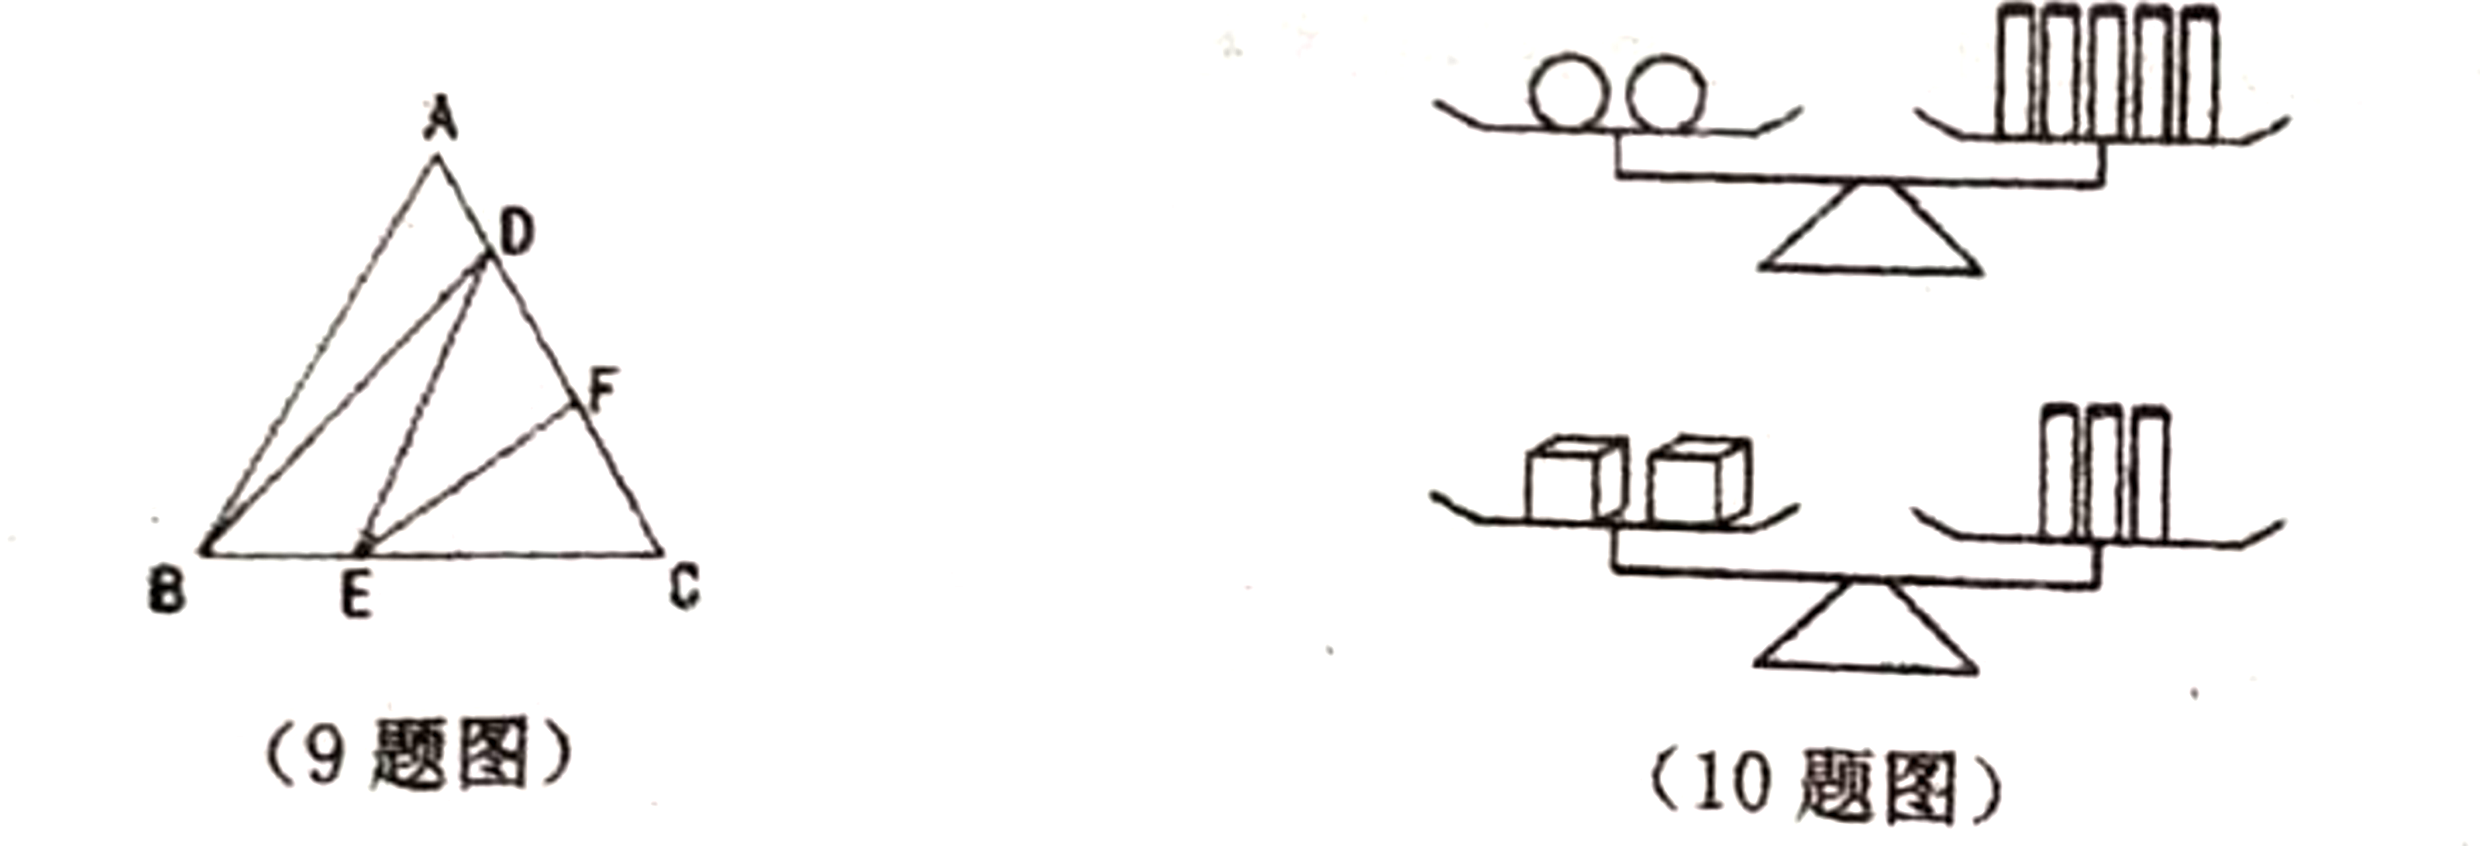
\includegraphics[width = 0.6\textwidth]{pic/1.9.png}
\end{figure}

10. 中央电视台二套“开心辞典”是一档广受大家喜爱的节目,某期有这样一个问题:如上右图所示,两个天平都平衡,根据图象回答三个球体的重量等于个(\qquad)正方体的重量。

11. 某班一次考试的平均分数是70分,其中的$\displaystyle \frac{3}{4}$人及格,他们的平均分是80分,则该班不及格的人的平均分是(\qquad)分。

\section{反复比较,择优录取:(共10分)}
1. 从镜子中能看到的左边图形是(\qquad)。
\begin{figure}[H]
    \centering
    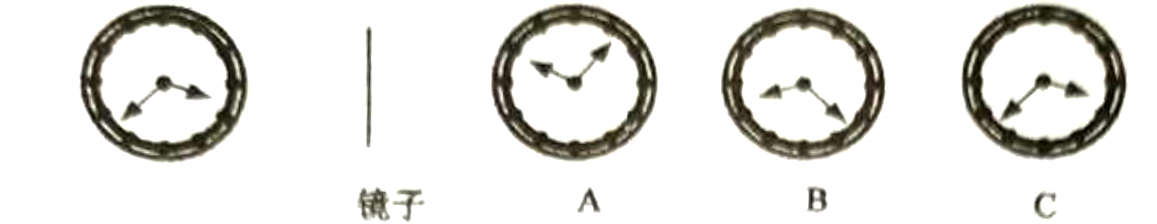
\includegraphics[width = 0.7\textwidth]{pic/2.1.png}
\end{figure}

2. 今年的四月二十四日是星期四,九月一日是星期(\qquad)。

A. 一;\qquad 
B. 二;\qquad 
C. 三;\qquad 
D. 四;\qquad 

3:一种直角三角形医用包扎巾,底是40厘米,高是30厘米,现有一块长240厘米,宽100厘米的长方形白布,最多可以做这样的包扎巾(不可以拼接)的块数是:(\qquad)。

B. 36\qquad 
C. 32\qquad 
D. 38\qquad 
A. 40\qquad 

4. 图1是一个三角形,沿虚线折叠后得到图2,这个多边形的面积是原三角形面积的$\displaystyle \frac{7}{9}$,己知图2中阴影部分的面积和为15平方厘米,那么原三角形的面积是(\qquad)平方厘米。
\begin{figure}[H]
    \centering
    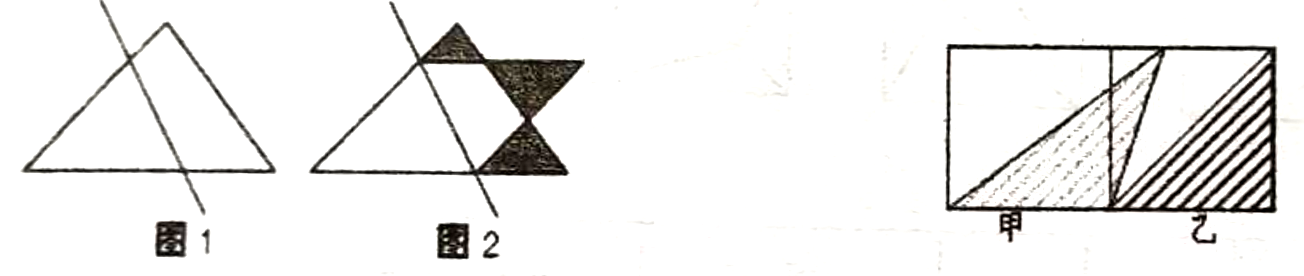
\includegraphics[width = 0.7\textwidth]{pic/2.4.png}
\end{figure}
A. 26\qquad 
B. 27\qquad 
C. 28\qquad 
D. 29\qquad 


5. 上右图,边长相等的两个正方形中,画了甲. 乙两个三角形(用阴影表示),它们的面积相比(\qquad)。

A. 甲的面积大\qquad 
B. 乙的面积大\qquad 
C. 相等\qquad 

\section{注意审题,巧思妙算:(写出主要计算过程)}
1. 计算下列个题:(共20分)

\vspace{12pt}
$\displaystyle 7.75\times 98\times 7\frac{3}{4}\times2$ \hspace{5cm}
$\displaystyle 2000-999\frac{3}{4}-99\frac{3}{4}-9\frac{3}{4}$

\vspace{3cm}
$\displaystyle 36.49 - 2\frac{15}{17} + 3.51 - 4\frac{2}{17}$\hspace{5cm}
$\displaystyle \frac{1}{2} + \frac{1}{4} + \frac{1}{8} + \frac{1}{16} + \frac{1}{16} + \frac{1}{32} + \frac{1}{64}$
\vspace{3cm}

2. 求未知数x。(共15分)

$6\times 3 - 1.8x=7.2$\hspace{3cm}
$2\times (2y-15)-10$\hspace{3cm}
$3.5x - 0.8x=54$

\vspace{3cm}

\section{自己探究,动手操作;(共15分)}

1. 在一个正方形的纸板内有若干个点(称为内点),用这些内点和正方形的4个顶点为三角形的顶点,能画出多少个不重叠的三角形?图中,分别画出了正方形内有一个内点. 两个内点. 三个内点的情形。(10分)
\begin{figure}[H]
    \centering
    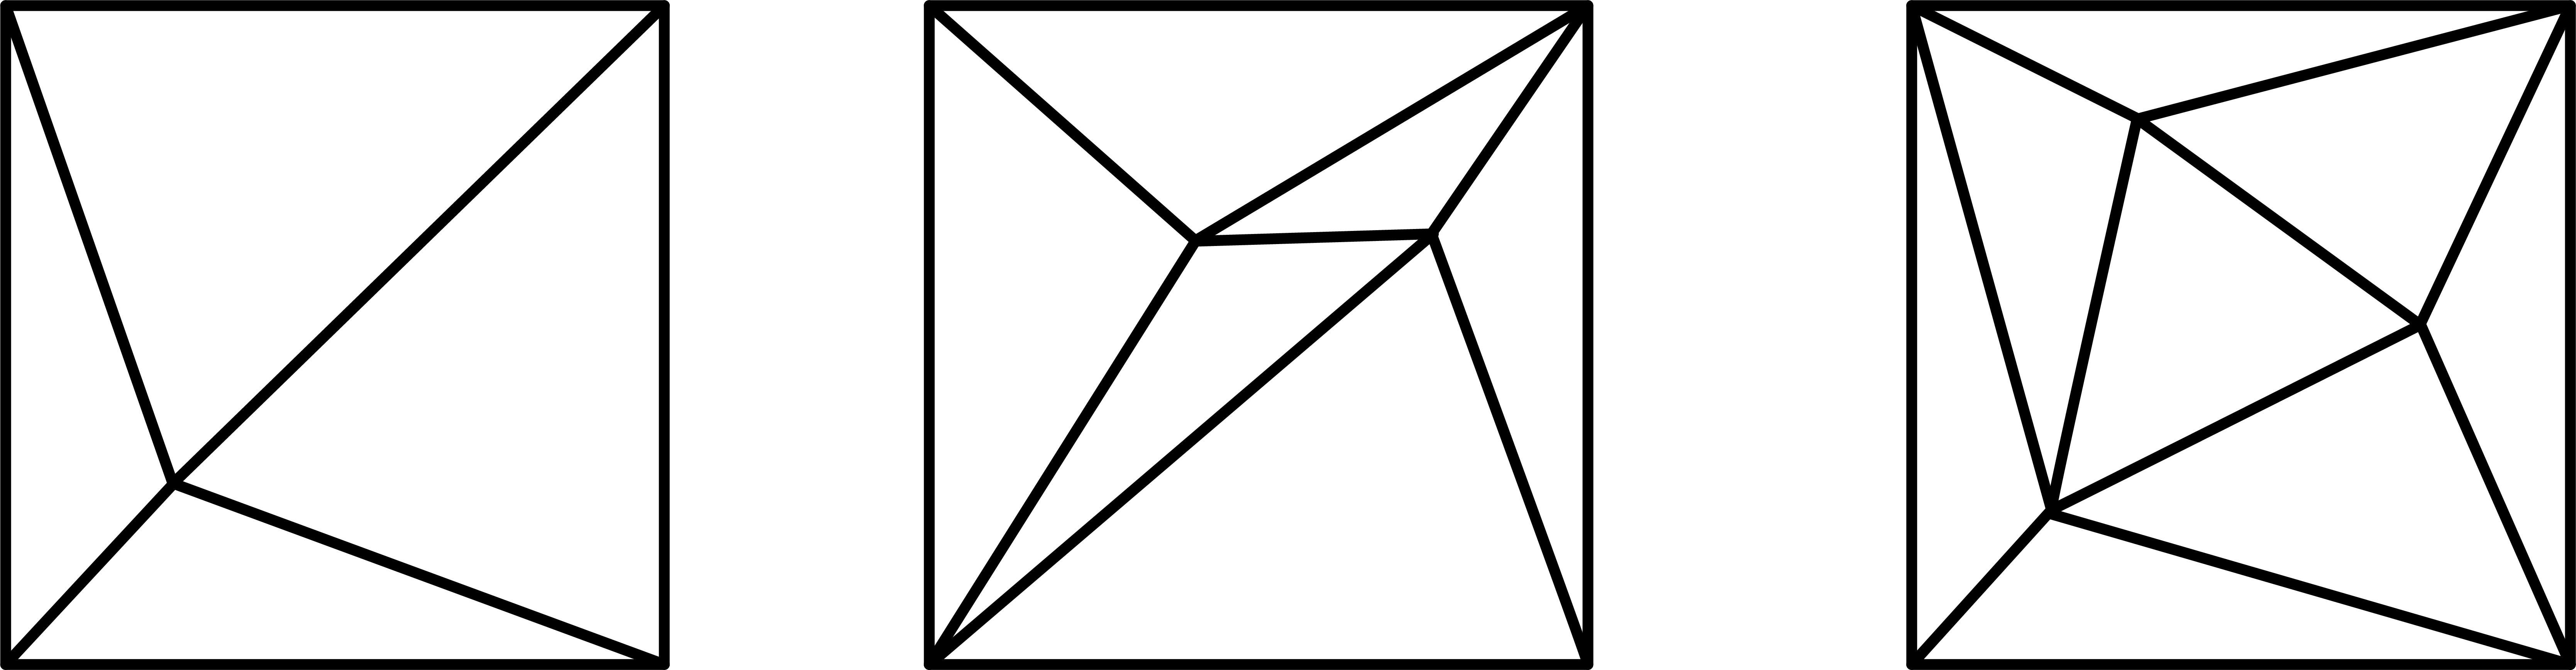
\includegraphics[width = 0.5\textwidth]{pic/4.1.png}
\end{figure}

(1)完成下表

    \begin{table}[H]
        \centering
        \setlength{\tabcolsep}{8mm}
        {\begin{tabular}{|c|c|c|c|}
            \hline
            内点个数 & 1 & 2 & 3 \\ \hline
            三角型个数 &  &  &  \\ \hline
        \end{tabular}}
    \end{table}
    
(2)正方形内有100个内点,能画出多少个不重叠的三角形?
\vspace{3cm}

2. 如图是边长6米的正方形和梯形拼成的“火炬”,梯形的上底长9米,A为上底的中点,B为下底的中点,线段AB恰好是梯形的高且长为3米,CD长为2米,那么,图中阴影部分的面积是多少平方米?(5分)
\begin{figure}[H]
    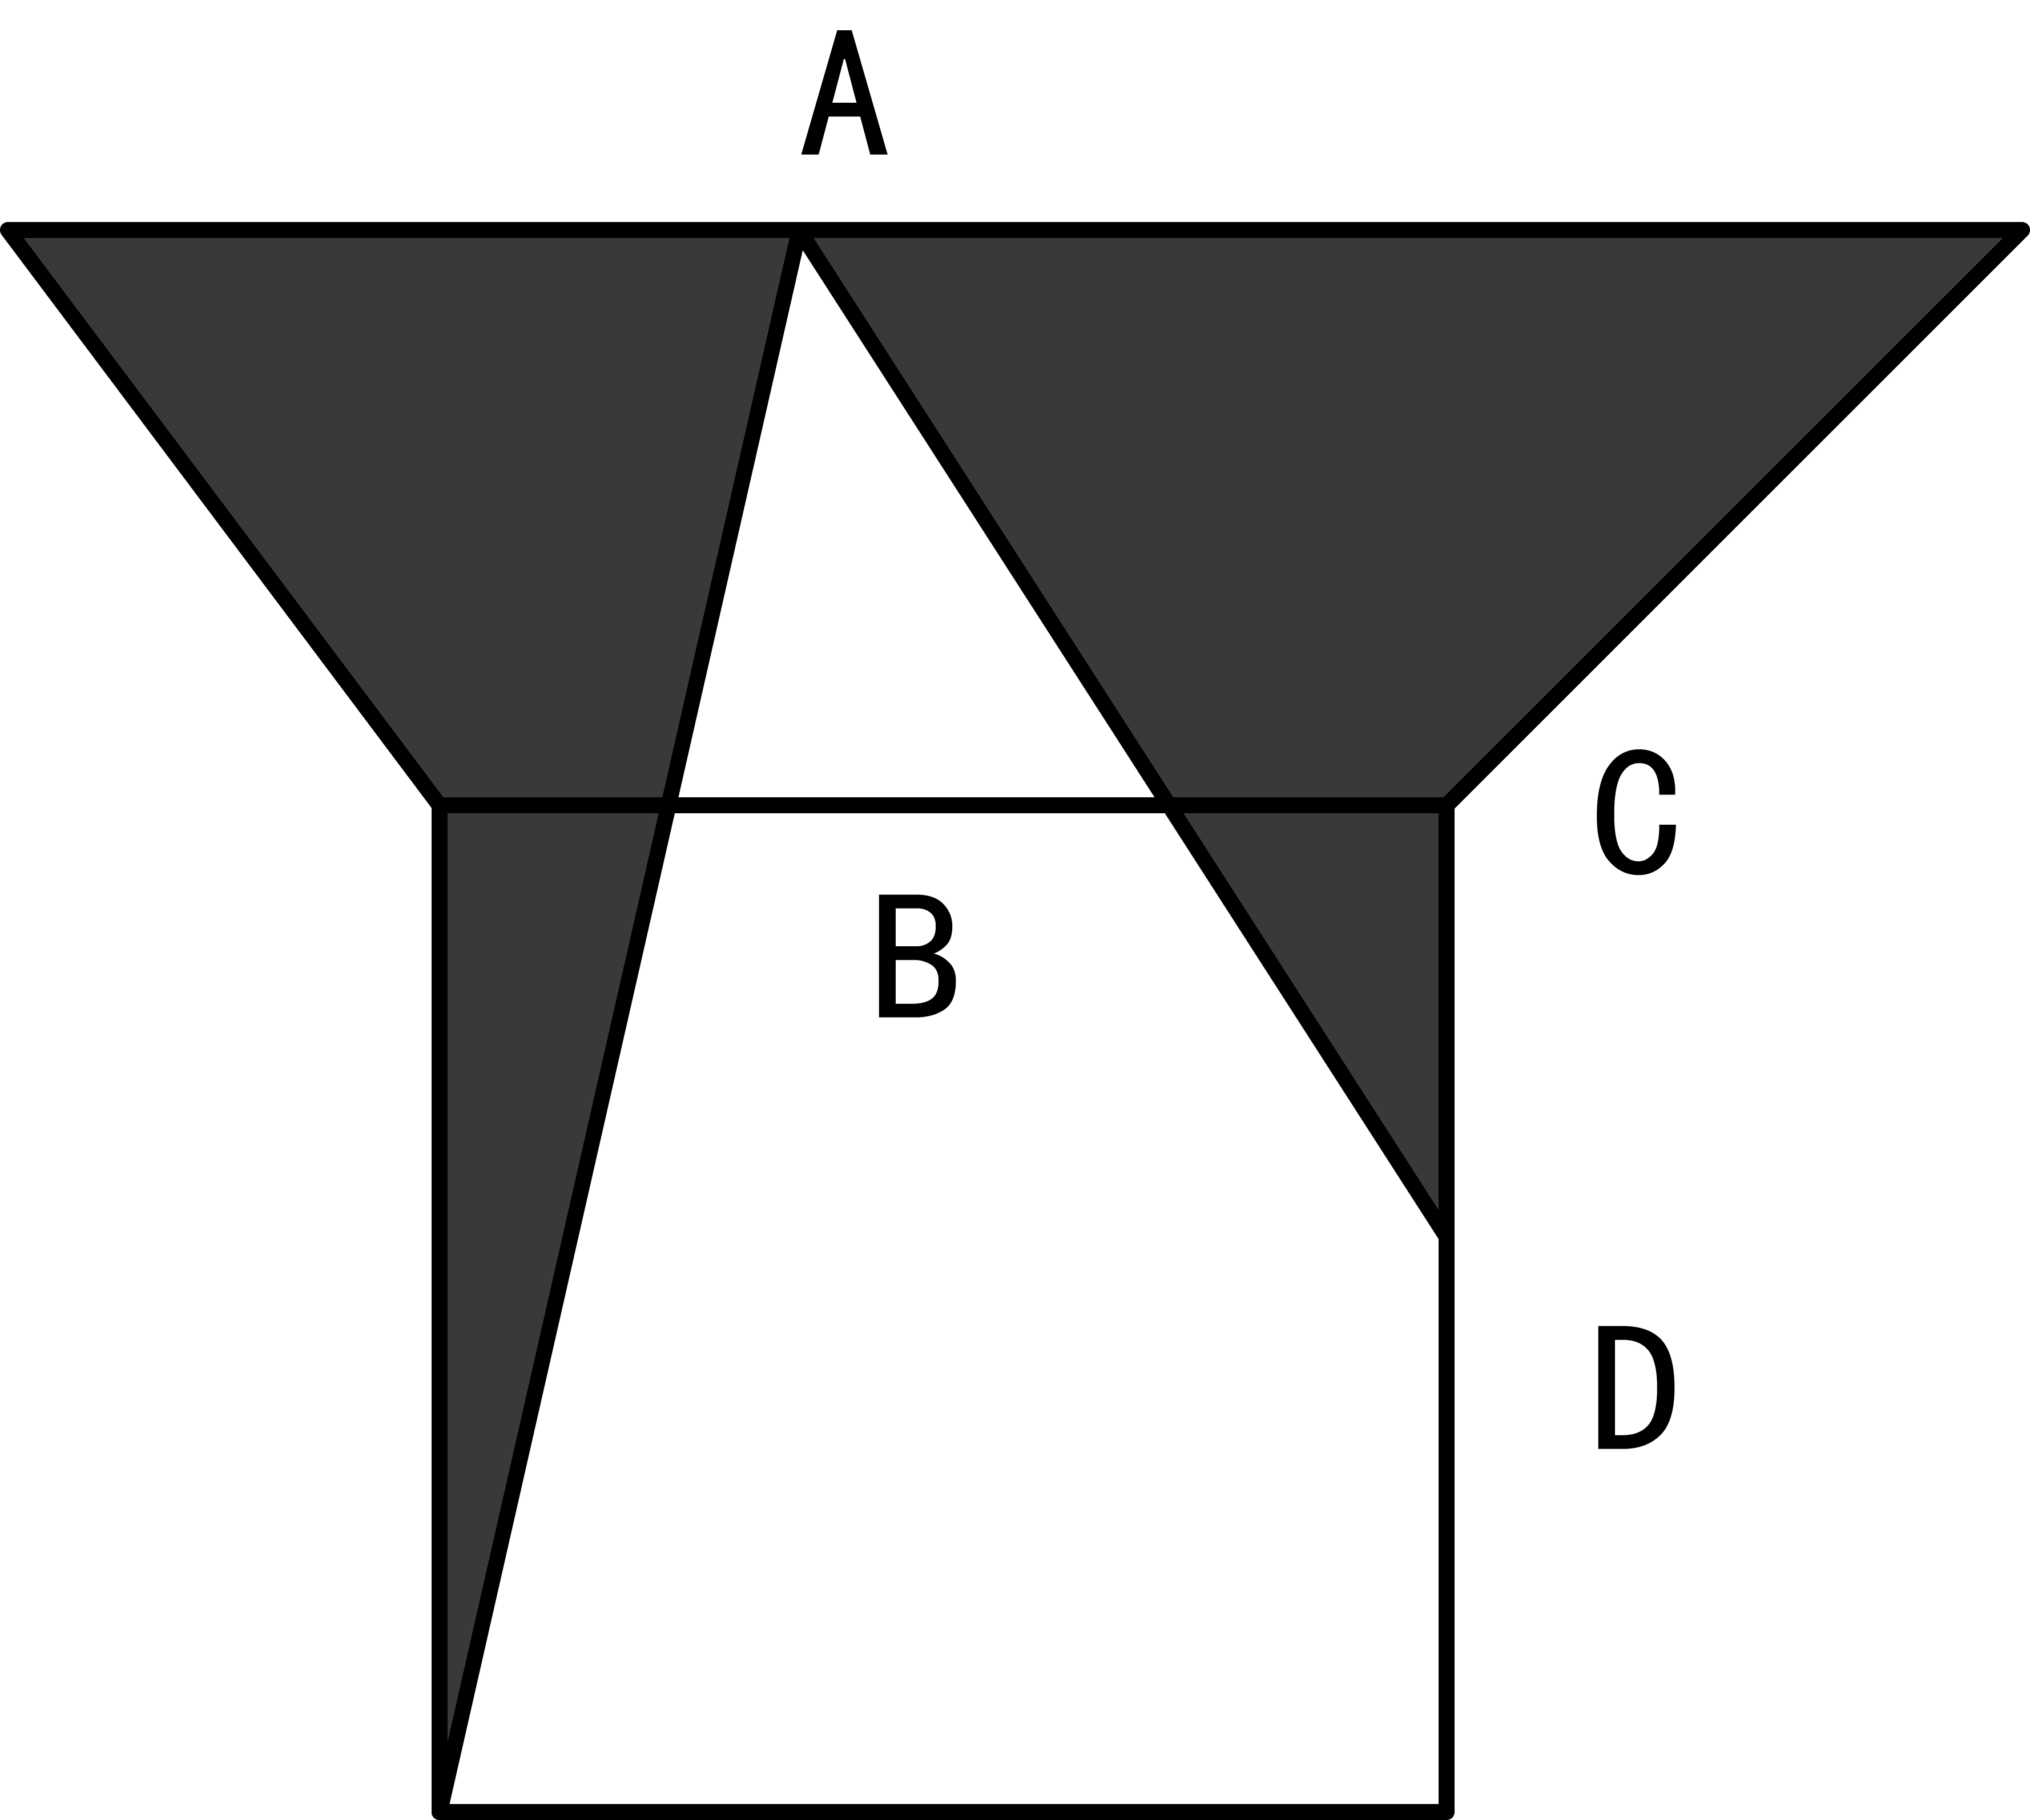
\includegraphics[width = 0.2\textwidth]{pic/4.2.png}
\end{figure}
% \vspace{3cm}

\section{解决问题:(共$6\times 6=36$分)}

1. 水果店上午卖出苹果53.6千克,下午卖出的苹果比上午卖出的1.2倍还多5.08千克。全天共卖出苹果多少千克?
\vspace{3cm}

2.一块麦田的形状如下图。麦田中间有一条2米宽的小路,按每平方米施肥0.1千克计算,这块田应施化肥多少干克?
\begin{figure}[H]
    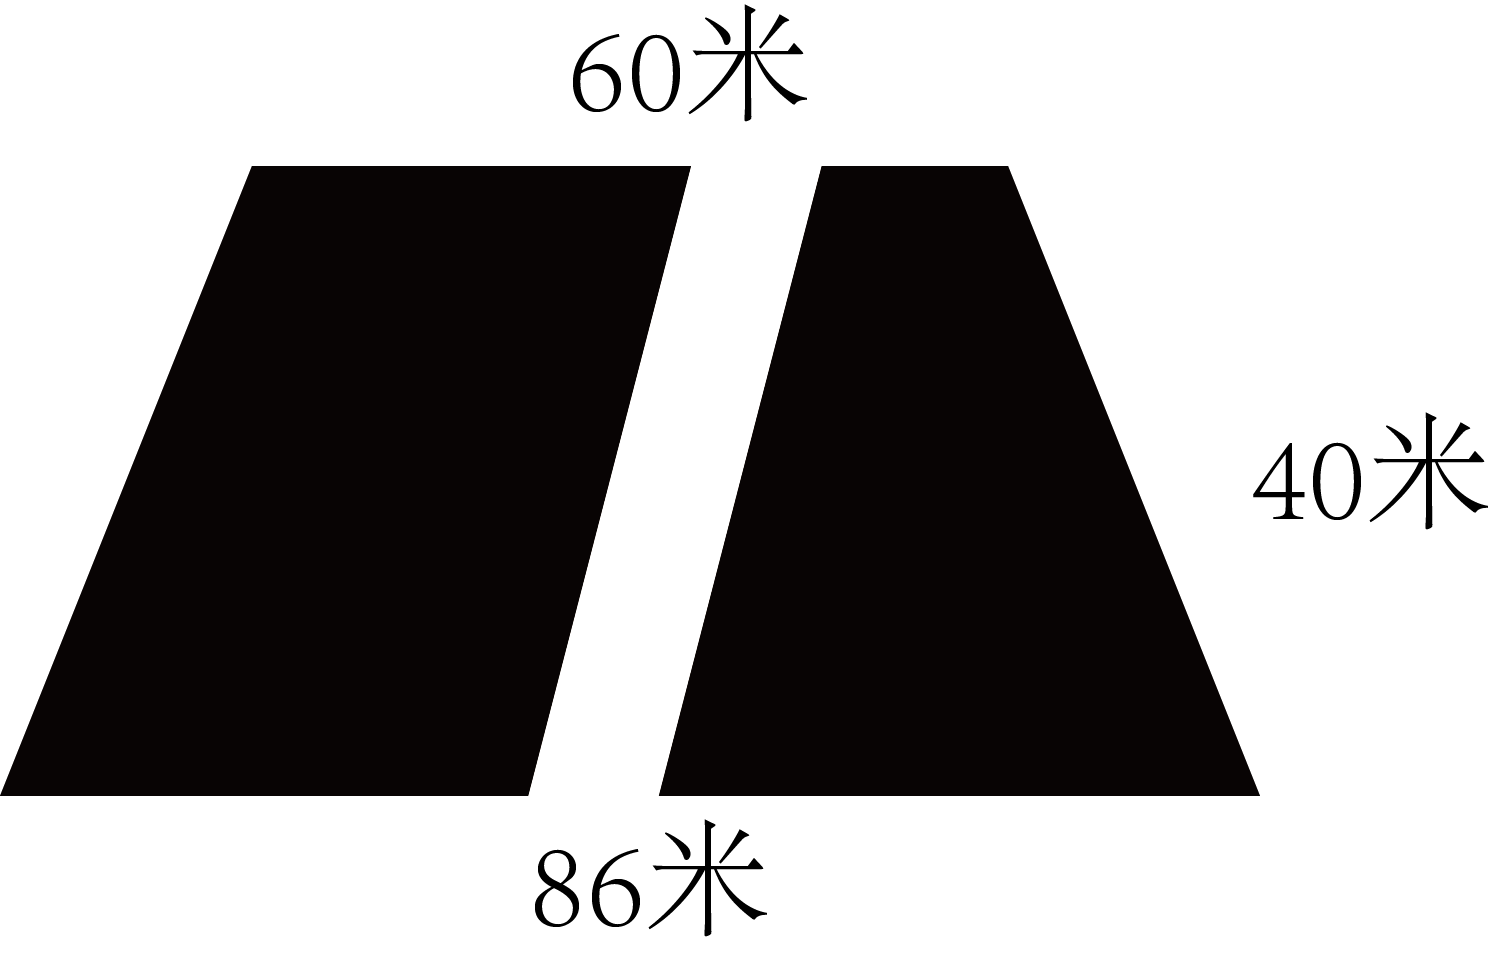
\includegraphics[width = 0.3\textwidth]{pic/5.2.png}
\end{figure}
\vspace{1CM}
3.某次大会安排住宿,若每间住2人,则有14人没有床位;若每间住3人,则多出2个空床位。问:宿舍共有几间?参加会议代表共几人?
\vspace{3cm}

4. 世界上最小的海是马尔马拉海,面积是1.1万平方千米,比我国太湖面积的4倍还多0.14万平方千米。我国太湖的面积是多少万平方千米?
\vspace{3cm}

5. 一辆汽车从甲地开往乙地,平均每小时行20千米。到乙地后又以每小时30千米的速度返回甲地,往返一次共用7.5小时。求甲. 乙两地间的路程。
\vspace{3cm}

6.甲船逆水航行300千米,需要15小时,返回原地需要10小时:乙船逆水航行同样的一段水路需要20小时,返回原地需要多少小时?
\vspace{3cm}

\setcounter{section}{0}
\setcounter{figure}{0}

\section{填空题(1-6小题每空1分,7-11每题2分共19分)}

1. 4立方米60立方分米=(\qquad)立方米 \hspace{2cm}2小时15分=(\qquad)时

2. 5÷1.1的商用循环小数的简便形式表示是3.自然数n-9相邻的较大的一个自然数是(\qquad)。

4. 一个小数由4个十和79个0.01组成,这个小数读作(\qquad)。

5. 2个人吃3个拼,每人吃到这些饼的$\displaystyle \frac{\mbox{()}}{\mbox{()}}$,也就是$\displaystyle \frac{\mbox{()}}{\mbox{()}}$个。

6.分数单位是$\displaystyle \frac{1}{10}$的所有最简真分数的和是(\qquad)。

7. 5个连续自然数的和是175,如果从小到大排列,那么排在最后的是(\qquad)。

8. 小明计算20道题目,规定做对一道题得5分,做错一道题反扣3分。小明20道题都做了,却只得了60分,问他做对了(\qquad)题。

9. 一盒饼干平均分给若干个小朋友,如果每人分4块,就多出3块;如果每人分6块,就少了5块。一共有(\qquad)个小朋友。

10. 一个六面都涂上红漆的大正方体的体积是27立方厘米,把它的切成27块1立方厘米的小正方体,小正方体任有一个面都没涂红漆的有(\qquad)块。

11. 把2个大小,,形状一样的直角梯形拼成一个平行四边形(但不是长方形),己知梯形的面积为60平方厘米,高为5厘米,一条腰长7厘米,拼成后的平行四边形的周长是(\qquad)厘米。

\section{选择题(在排号内填入正确答案的字母番号。每题2分,共10分)}

1. 一个三角形与一个平行四边形的底和面积都相等,已知平行四边形的高是8厘米,那么三角形的高是(\qquad)

A. 4厘米\qquad
B. 8厘米\qquad
C. 16厘米\qquad 
D. 32厘米

2. 4.27÷1.9商取2.2时,剩余部分是(\qquad)

A. 9\qquad 
B. 0.9\qquad 
C. 0. 09\qquad 
D. 0.009\qquad 

3. 一个正六边形(如右图),它有(\qquad)条对称轴。

A. 3\qquad
B. 4\qquad
C. 5\qquad
D. 6\qquad

4.已知m=4n(m,n不为0),那么m和n的最大公因数是(\qquad)

A. m\qquad
B. n\qquad
C. 4\qquad
D. 无法确定\qquad

5. 用8块1立方厘米的正方体积木搭长方体,可以搭出(\qquad)长方体(包括正方体)

A. 2\qquad
B. 3\qquad
C. 4\qquad
D. 5\qquad

\section{计算(24分)}

1. 能简算的请简算(15运分)

$12.25 - 7.85 - 2.15 + 7.75$
\hspace{3cm}
$(4+8)\times 25\times 128$
\hspace{3cm}
$6+7+8+…+34+35$

\vspace{3cm}

$201.6\times 3.24+20.16\times 77.6-201.6$
\hspace{5cm}
$\displaystyle \frac{1}{2} + \frac{1}{4} + \frac{1}{8} + \frac{1}{16} + \frac{1}{32} + \frac{1}{64} + \frac{1}{128} $

\vspace{3cm}

2. 解方程:(9分)

$2x+4=12.5$\hspace{3cm}
$17.28 - 4(x-2) = 5.28$\hspace{3cm}
$2.8 \div (3x-2.5)=2$
\vspace{3cm}


\section{探究计算〈共17分)}

1. 如图:一条直线最多可以将一个长方形分成2部分,两条直线最多可以将一个长方形分成4
部分:(6分)

(1)画一画3条直线,最多可以将一个长方形分成(\qquad)部分
(2)4条直现最多可以将一个长方形分成(\qquad)部分
(3)若长方形被分成了46个部分,则最少需要(\qquad)条直线

2. 如图:小正方形和大正方形的对角线分别长1.4厘米和3.6厘米.梯形ABCD 的面积是多少?(5分)

3. 如图:长方形 ABCD 的面积是180平方分米,三角形DOE的面积是22.5平方分米,DO=7.5分米(5分)

求:(1)三角形AOD的面积;(3分)

(2)CE的长度。(3分)

\section{解决问题。(30分)}

1. 家具厂订购500根方木,每根方木横截面的面积是2.4平方分米,长是3米。这些木料一排多少方?

2. 某人工作一年的酬金是18000元和一台全自动洗衣机。他干了7个月,得到了8400元和一台全自动洗衣机。请问这台全自动洗衣机值多少元?

3. 从学校到少年宫的这段公路上,一共有37根电线杆,原来每两根电线杆之间相距50米,现在要改成每两根乙间相距60米,除了两端两根不需移动外,中途还有多少根不必移动?

4. 甲仓库有大米370袋,乙仓库有大米280袋,从甲仓库运出多少袋大米后,乙仓库的大米正好是甲仓库大米的4倍?

5. 小明和小胖同时从学校到少年宫去,小明每分钟走80米,小胖每分钟走60米,小明从学校到少年宫走了7分钟,到少年宫发现忘带东西了立即返回,在返回途中碰到小胖,问小

胖从学校出发经过几分钟和小明在途中相遇?
6. 给定6个数:1,3,9,27,81,243。从这6个数中每次取n个数求和(每个数只能取1次),可以得到1个新数,这样共可得到63个新数,把它们按从小到大依次排列起来是1,3,4,9,10,12,13,27....请问:第60个数是多少?



\end{document}